\documentclass{article}
\usepackage{xeCJK}
\usepackage{fancyhdr}
\usepackage{extramarks}
\usepackage{amsmath}
\usepackage{amsthm}
\usepackage{amsfonts}
\usepackage{tikz}
\usepackage[plain]{algorithm}
\usepackage{algpseudocode}
\usepackage{datetime}
\usetikzlibrary{automata,positioning}

%
% 基本设置
%

\topmargin=-0.45in
\evensidemargin=0in
\oddsidemargin=0in
\textwidth=6.5in
\textheight=9.0in
\headsep=0.25in

\linespread{1.1}

\pagestyle{fancy}
\lhead{\small{\hmwkAuthorName} \\ \small{\hmwkAuthorClass 班}} % 页眉左侧
\chead{\hmwkClass\ : \hmwkTitle} % 页眉中间
\rhead{\firstxmark} % 页眉右侧
\lfoot{\lastxmark} % 页脚左侧
\cfoot{\thepage}  % 页脚中间

\renewcommand\headrulewidth{1pt}
\renewcommand\footrulewidth{0.4pt}

\setlength\parindent{0pt}

%
% 题目相关设置
%

\newcommand{\enterProblemHeader}[1]{
    \nobreak\extramarks{}{题目 \arabic{#1} continued on next page\ldots}\nobreak{}
    \nobreak\extramarks{题目 \arabic{#1} (continued)}{题目 \arabic{#1} continued on next page\ldots}\nobreak{}
}

\newcommand{\exitProblemHeader}[1]{
    \nobreak\extramarks{题目 \arabic{#1} (continued)}{题目 \arabic{#1} continued on next page\ldots}\nobreak{}
    \stepcounter{#1}
    \nobreak\extramarks{题目 \arabic{#1}}{}\nobreak{}
}

\setcounter{secnumdepth}{0}
\newcounter{partCounter}
\newcounter{homeworkProblemCounter}
\setcounter{homeworkProblemCounter}{1}
\nobreak\extramarks{题目 \arabic{homeworkProblemCounter}}{}\nobreak{}

%
% Homework Problem Environment
% 这个环境有一个可选的参数, 当给出这个参数的时候可以调整题目计数器, 适合用在
% 题号不连续的情况.例子在最后一页.
%
\newenvironment{homeworkProblem}[1][-1]{
    \ifnum#1>0
        \setcounter{homeworkProblemCounter}{#1}
    \fi
    \section{题目 \arabic{homeworkProblemCounter}}
    \setcounter{partCounter}{1}
    \enterProblemHeader{homeworkProblemCounter}
}{
    \exitProblemHeader{homeworkProblemCounter}
}


\renewcommand{\part}[1]{\textbf{\large Part \Alph{partCounter}}\stepcounter{partCounter}\\}
\renewcommand{\today}{\number\year 年 \number\month 月 \number\day 日} 
\renewcommand{\proofname}{证明}
\renewcommand{\figurename}{图}
\floatname{algorithm}{算法}

\makeatletter \renewenvironment{proof}[1][\proofname]{\par     \pushQED{\qed}%
\normalfont \topsep6\p@\@plus6\p@ \labelsep1em\relax     \trivlist     \item[\hskip\labelsep\indent \bfseries #1]\ignorespaces }{%
\popQED\endtrivlist\@endpefalse } \makeatother

\newcommand{\hmwkTitle}{作业 \ 2}
\newcommand{\hmwkDueDate}{1919  年 8  月 \ 10  日}
\newcommand{\hmwkClass}{占卜学}
\newcommand{\hmwkClassTime}{}
\newcommand{\hmwkClassInstructor}{}
\newcommand{\hmwkAuthorID}{114514}
\newcommand{\hmwkAuthorClass}{计算机 1919}
\newcommand{\hmwkAuthorName}{李田所}

%
% 标题页
%

\title{
    \vspace{2in}
    \textmd{\textbf{\hmwkClass:\ \hmwkTitle}}\\
    \normalsize\vspace{0.1in}\small{截止时间: \ \hmwkDueDate}\\
    \vspace{0.1in}\large{\textit{\hmwkClassInstructor\ \hmwkClassTime}}
    \vspace{3in}
}

\author{ \hmwkAuthorClass 班\\ \hmwkAuthorName \\ 学号: \hmwkAuthorID }
\date{\today}

% 算法
\newcommand{\alg}[1]{\textsc{\bfseries \footnotesize #1}}

% 导数
\newcommand{\deriv}[1]{\frac{\mathrm{d}}{\mathrm{d}x} (#1)}

% 偏导数
\newcommand{\pderiv}[2]{\frac{\partial}{\partial #1} (#2)}

% dx(微积分)
\newcommand{\dx}{\mathrm{d}x}

\newcommand{\solution}{\textbf{\large 解:}}
\newcommand{\pf}{\textbf{\large 证明:}}

% 概率: 期望, 方差, 协方差, 偏差
\newcommand{\E}{\mathrm{E}}
\newcommand{\Var}{\mathrm{Var}}
\newcommand{\Cov}{\mathrm{Cov}}
\newcommand{\Bias}{\mathrm{Bias}}

\begin{document}

\maketitle

\pagebreak

\begin{homeworkProblem}
    求一个合适的整数 \(c\) ,使得 \(f(n) \leq c \cdot
    g(n)\) 对 \(n > 1\) 恒成立.

    \begin{enumerate}
        \item \(f(n) = n^2 + n + 1\), \(g(n) = 2n^3\)
        \item \(f(n) = n\sqrt{n} + n^2\), \(g(n) = n^2\)
        \item \(f(n) = n^2 - n + 1\), \(g(n) = n^2 / 2\)
    \end{enumerate}

    \solution

    显然地, 我们可以通过占卜法来解c的值
    \(c\).
    \\

    \textbf{1.}

    \[
        \begin{split}
            n^2 + n + 1 &=
            \\
            &\leq n^2 + n^2 + n^2
            \\
            &= 3n^2
            \\
            &\leq c \cdot 2n^3
        \end{split}
    \]

    故 \(c = 2\) 满足要求.
    \\

    \textbf{2.}

    \[
        \begin{split}
            n^2 + n\sqrt{n} &=
            \\
            &= n^2 + n^{3/2}
            \\
            &\leq n^2 + n^{4/2}
            \\
            &= n^2 + n^2
            \\
            &= 2n^2
            \\
            &\leq c \cdot n^2
        \end{split}
    \]

    故 \(c = 2\) 满足要求.
    \\

    \textbf{3.}

    \[
        \begin{split}
            n^2 - n + 1 &=
            \\
            &\leq n^2
            \\
            &\leq c \cdot n^2/2
        \end{split}
    \]

    故 \(c = 2\) 满足要求.

\end{homeworkProblem}

\pagebreak

\begin{homeworkProblem}
    令 \(\Sigma = \{0, 1\}\).建立一个有限状态自动机 \(A\) 来识别可以被 5 整除的二进制串.
    \\

    令状态 \(q_k\) 表示\(k\)被5除的余数. 例如,7 对应 \(q_2\) (因为 \(7
    \mod 5 = 2\) ).

    \begin{figure}[h]
        \centering
        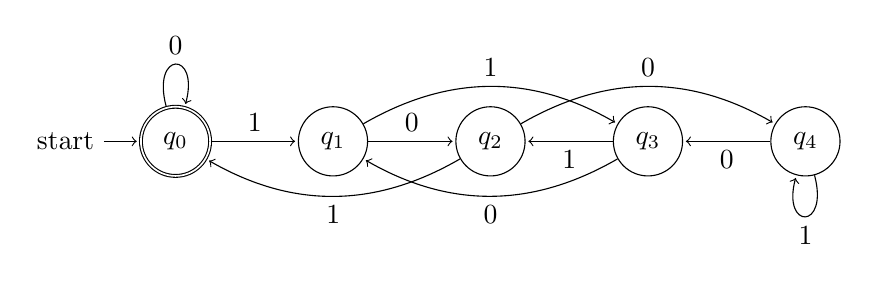
\begin{tikzpicture}[shorten >=1pt,node distance=2cm,on grid,auto]
            \node[state, accepting, initial] (q_0)   {$q_0$};
            \node[state] (q_1) [right=of q_0] {$q_1$};
            \node[state] (q_2) [right=of q_1] {$q_2$};
            \node[state] (q_3) [right=of q_2] {$q_3$};
            \node[state] (q_4) [right=of q_3] {$q_4$};
            \path[->]
                (q_0)
                    edge [loop above] node {0} (q_0)
                    edge node {1} (q_1)
                (q_1)
                    edge node {0} (q_2)
                    edge [bend right=-30] node {1} (q_3)
                (q_2)
                    edge [bend left] node {1} (q_0)
                    edge [bend right=-30] node {0} (q_4)
                (q_3)
                    edge node {1} (q_2)
                    edge [bend left] node {0} (q_1)
                (q_4)
                    edge node {0} (q_3)
                    edge [loop below] node {1} (q_4);
        \end{tikzpicture}
        \caption{DFA \  \(A\) \ 真好看, 是不是?}
        \label{fig:multiple5}
    \end{figure}

    \textbf{解释}
    \\

    给出一个二进制表示的数, \(x\).由于我们的状态机只接受两种输入, \(x\) can either become \(x0\) or \(x1\). When a 0 comes
    into the state machine, it is the same as taking the binary number and
    multiplying it by two. When a 1 comes into the machine, it is the same as
    multipying by two and adding one.
    \\

    通过这一点, 我们就可以建立出一个转移表:

    \begin{table}[ht]
        \centering
        \begin{tabular}{c || c | c | c | c | c}
            & \(x \mod 5 = 0\)
            & \(x \mod 5 = 1\)
            & \(x \mod 5 = 2\)
            & \(x \mod 5 = 3\)
            & \(x \mod 5 = 4\)
            \\
            \hline
            \(x0\) & 0 & 2 & 4 & 1 & 3 \\
            \(x1\) & 1 & 3 & 0 & 2 & 4 \\
        \end{tabular}
    \end{table}

    Therefore on state \(q_0\) or (\(x \mod 5 = 0\)), a transition line should
    go to state \(q_0\) for the input 0 and a line should go to state \(q_1\)
    for input 1. Continuing this gives us the Figure~\ref{fig:multiple5}.
\end{homeworkProblem}

\begin{homeworkProblem}
    写出快速排序算法的一部分 \alg{Quick-Sort($list, start, end$)}

    \begin{algorithm}[]
        \begin{algorithmic}[1]
            \Function{Quick-Sort}{$list, start, end$}
                \If{$start \geq end$}
                    \State{} \Return{}
                \EndIf{}
                \State{} $mid \gets \Call{Partition}{list, start, end}$
                \State{} \Call{Quick-Sort}{$list, start, mid - 1$}
                \State{} \Call{Quick-Sort}{$list, mid + 1, end$}
            \EndFunction{}
        \end{algorithmic}
        \caption{快速排序的开始部分}
    \end{algorithm}
\end{homeworkProblem}

\pagebreak

\begin{homeworkProblem}
    假设我们想要拟合一条过原点的直线, 如,
    \(Y_i = \beta_1 x_i + e_i\) 其中 \(i = 1, \ldots, n\), \(\E [e_i] = 0\),
     \(\Var [e_i] = \sigma^2_e\) and \(\Cov[e_i, e_j] = 0, \forall i \neq
    j\).
    \\

    \part

    Find the least squares esimator for \(\hat{\beta_1}\) for the slope
    \(\beta_1\).
    \\

    \solution

    To find the least squares estimator, we should minimize our Residual Sum
    of Squares, RSS:

    \[
        \begin{split}
            RSS &= \sum_{i = 1}^{n} {(Y_i - \hat{Y_i})}^2
            \\
            &= \sum_{i = 1}^{n} {(Y_i - \hat{\beta_1} x_i)}^2
        \end{split}
    \]

    By taking the partial derivative in respect to \(\hat{\beta_1}\), we get:

    \[
        \pderiv{
            \hat{\beta_1}
        }{RSS}
        = -2 \sum_{i = 1}^{n} {x_i (Y_i - \hat{\beta_1} x_i)}
        = 0
    \]

    This gives us:

    \[
        \begin{split}
            \sum_{i = 1}^{n} {x_i (Y_i - \hat{\beta_1} x_i)}
            &= \sum_{i = 1}^{n} {x_i Y_i} - \sum_{i = 1}^{n} \hat{\beta_1} x_i^2
            \\
            &= \sum_{i = 1}^{n} {x_i Y_i} - \hat{\beta_1}\sum_{i = 1}^{n} x_i^2
        \end{split}
    \]

    Solving for \(\hat{\beta_1}\) gives the final estimator for \(\beta_1\):

    \[
        \begin{split}
            \hat{\beta_1}
            &= \frac{
                \sum {x_i Y_i}
            }{
                \sum x_i^2
            }
        \end{split}
    \]

    \pagebreak

    \part

    Calculate the bias and the variance for the estimated slope
    \(\hat{\beta_1}\).
    \\

    \solution

    For the bias, we need to calculate the expected value
    \(\E[\hat{\beta_1}]\):

    \[
        \begin{split}
            \E[\hat{\beta_1}]
            &= \E \left[ \frac{
                \sum {x_i Y_i}
            }{
                \sum x_i^2
            }\right]
            \\
            &= \frac{
                \sum {x_i \E[Y_i]}
            }{
                \sum x_i^2
            }
            \\
            &= \frac{
                \sum {x_i (\beta_1 x_i)}
            }{
                \sum x_i^2
            }
            \\
            &= \frac{
                \sum {x_i^2 \beta_1}
            }{
                \sum x_i^2
            }
            \\
            &= \beta_1 \frac{
                \sum {x_i^2 \beta_1}
            }{
                \sum x_i^2
            }
            \\
            &= \beta_1
        \end{split}
    \]

    Thus since our estimator's expected value is \(\beta_1\), we can conclude
    that the bias of our estimator is 0.
    \\

    For the variance:

    \[
        \begin{split}
            \Var[\hat{\beta_1}]
            &= \Var \left[ \frac{
                \sum {x_i Y_i}
            }{
                \sum x_i^2
            }\right]
            \\
            &=
            \frac{
                \sum {x_i^2}
            }{
                \sum x_i^2 \sum x_i^2
            } \Var[Y_i]
            \\
            &=
            \frac{
                \sum {x_i^2}
            }{
                \sum x_i^2 \sum x_i^2
            } \Var[Y_i]
            \\
            &=
            \frac{
                1
            }{
                \sum x_i^2
            } \Var[Y_i]
            \\
            &=
            \frac{
                1
            }{
                \sum x_i^2
            } \sigma^2
            \\
            &=
            \frac{
                \sigma^2
            }{
                \sum x_i^2
            }
        \end{split}
    \]

\end{homeworkProblem}

\pagebreak

\begin{homeworkProblem}
    证明一个\(k\) 阶的多项式, \(a_kn^k + a_{k - 1}n^{k - 1} + \hdots
    + a_1n^1 + a_0n^0\) 是 \(\Theta(n^k)\) 的, 其中 \(a_k \hdots a_0\)
    都是非负常数.

    \begin{proof}
        为了证明 \(a_kn^k + a_{k - 1}n^{k - 1} + \hdots + a_1n^1 +
        a_0n^0\), 只需证明:

        \[
            \exists c_1 \exists c_2 \forall n \geq n_0,\ {c_1 \cdot g(n) \leq
            f(n) \leq c_2 \cdot g(n)}
        \]

        对于第一个不等式, 显然它是成立的. 因为无论常数是何值, \(n^k \leq a_kn^k + a_{k - 1}n^{k - 1} +
        \hdots + a_1n^1 + a_0n^0\) even if \(c_1 = 1\) and \(n_0 = 1\).  
        这是因为又 \(n^k \leq c_1 \cdot a_kn^k\) 对任意的常数
        \(c_1\) 和 \(a_k\).
        \\

        对于第二个不等式, 我们可以这样证明:
        记 \(A\) \(=\)  \(\sum\limits_{i=0}^k a_i\) , 则有,

        \[
            \begin{split}
                a_kn^k + a_{k - 1}n^{k - 1} + \hdots + a_1n^1 + a_0n^0 &=
                \\
                &\leq (a_k + a_{k - 1} \hdots a_1 + a_0) \cdot n^k
                \\
                &= A \cdot n^k
                \\
                &\leq c_2 \cdot n^k
            \end{split}
        \]

        其中 \(n_0 = 1\) 和 \(c_2 = A\). \(c_2\) 是常数. 这就证明了结论.
    \end{proof}
\end{homeworkProblem}

\pagebreak

%
% 编号不连续的情况
%

% 用参数跳到18
\begin{homeworkProblem}[18]
    比较 \(\sum_{k=1}^{5} k^2\) 和 \(\sum_{k=1}^{5} (k - 1)^2\).
\end{homeworkProblem}

% 不带参数继续计数(19)
\begin{homeworkProblem}
    求 \(f(x) = x^4 + 3x^2 - 2\) 的导数.
\end{homeworkProblem}

% 再次修改参数
\begin{homeworkProblem}[6]
    计算定积分
    \(\int_0^1 (1 - x^2) \dx\)
    和
    \(\int_1^{\infty} \frac{1}{x^2} \dx\).
\end{homeworkProblem}

\end{document}
